\chapter{Discussion}
\label{chap:discussion}
In this chapter, the research results are discussed and contextualized with the research questions (see Chapter \ref{chap:introduction}) and the idea that inspired this work: evaluating the feasibility of performing real-time Emotion-Recognition with a wearable device for a future affective \ac{BCI} system. 

\section{Challenges towards real-time Emotion-Recognition}
\label{sec:challenges}
When imagining users adopting a technology in their life, many functional and design aspects are rightfully expected. For example, the design of the device needs to be sleek and intuitive, and the flow of the application must be seamlessly integrated and well performing. This is clearly not the case for current Brain-Computer Interfaces, that are still in their infancy and far from mass adoption, especially for non-clinical applications. Lin, Jung and Onton \cite{lin_toward_2015} reviewed a collection of methods that could greatly improve the quality of the user experience and finally open the way for affective \ac{BCI} to reach the consumer market. The core challenge of affective \ac{BCI}  is to create a plug-and-play \ac{BCI}  system with limited electrodes that can consistently perform accurate Emotion-Recognition regardless of the person that is using it. The other challenges consequently follow:
\begin{itemize}
\item 	\textbf{Reduction and selection of electrodes:} the number of electrodes must be relatively small, between 2 and 8, and strategically placed over the cortical areas delegated to the processing of emotions. They also should be soft dry electrodes and the system should be able to automatically recognize bad channels and excluding them from the processing.
\item 	\textbf{Automatic artifacts cleaning}: artefacts are one of the most impacting problems, and currently the most popular approaches for offline artifact cleaning are \ac{ICA}, that is not applicable to small sets of electrodes and too computationally expensive for online cleaning, and visual inspection. Alternative approaches might be achieved using regression to train algorithms in recognizing specific types of artifacts or features of the signal that indicate whether the quality is good or not and adjust it accordingly. Cleaning artifacts is also vital to the efficient use of as much data as possible. In the current study the artifacts removal strategy led to the exclusion of 10 participants and the removal of up to 25\% of the data of the remaining participants, a considerable cost considering the time and efforts needed to collect the data with an experimental protocol.
\item 	\textbf{Features selection and reduction}: selecting the most suitable features allows to reduce the computational cost by removing redundant and less meaningful features, and this is particularly correlated to the selection of electrodes as well. Lin et al. \cite{lin_toward_2015} through their extensive research over the years discovered that differential asymmetries are the most consistent type of features among subjects and sessions, reliable also for subject-independent classification. In more recent studies, Thammasan et al. \cite{thammasan_continuous_2016}, Keelawat et al \cite{keelawat_comparative_2021} and Avramidis et al. \cite{avramidis_multiscale_2021} , extracted \ac{EEG} features using fractal dimension algorithms instead of \ac{PSD}, obtaining significantly better performances in both subject-dependent and subject-independent classification. Another possibility is to use more complex models like \ac{CNN} \cite{keelawat_comparative_2021} to automatically extract features from the \ac{EEG} signal, sacrificing the ease of interpretability of the model and the direct connection with the theoretical neuroscience.
\item 	\textbf{Users training and calibration}: a very time consuming and frustrating process is the calibration of \ac{BCI} systems for new users, especially if they have no experience of brain-controlled inputs. A system that can only classify emotions with a subject-dependent strategy is bound to train the users in reporting their emotions and then train a classifier with the collected data, all under the assumption that the resulting dataset is not too unbalanced. This of course is not feasible, and ultimately subject-independent classification should be the aim for real-time systems. However, this might not suffice, and even subject-independent classifiers might have to be tuned with short calibration sessions to adjust for each specific case, for example by selecting more susceptible features for a certain user that matches similar brain “signatures” from a group of users that the model has already been trained on. Zero-training strategies \cite{krauledat_towards_2008,jeong_hybrid_2021} have been object of study over the last decade and using spatial filters and transfer learning makes it possible to train a sub-optimal decoder and then use unsupervised learning to transform it into a user specific decoder. Of course, these solutions are still very experimental and use case specific, and further investigation is required.
\end{itemize}

The rest of the chapter will contextualize these challenges in the current study. Using a wearable EEG is a solution to the first problem, but also a constraint around which every other problem had to be worked around.

\section{Self-reported emotional labels}
\label{sec:self_reported_labels}
Reporting emotions is a non-trivial task and could be subjectively difficult. From the feedback forms collected after the experiment, 7 subjects reported to have found difficulties in choosing the quadrant of the valence-arousal space, 8 subjects reported difficulties in assessing the emotional intensity (in both dimensions) and 9 subjects reported difficulties in assessing the specific emotions. In addition, participants reported an average fatigue score of 2.47 ± 0.97 after the first half of the experiment and a fatigue score of 3.27 ± 0.86, on a scale from 1 to 5. Some emotions were reported to be missing from the simplified valence-arousal space, for example "annoyance". Another missing emotion was “bittersweet”, that is commonly experienced in music listening yet difficult to report because of its composition of not-adjacent emotions (sadness, happiness) on the valence-arousal space. Continuous annotation of emotions has several advantages over discrete annotation, allowing a more granular reporting that consider emotional “oscillations” over the duration of a stimulus and more distributed labels across all classes that can favor the classification task.  It is a powerful tool for researchers to build affective datasets but heading towards a real product it will eventually be an obstacle as it requires an extra layer of training before the calibration. Discrete annotations are a simpler task that has virtually no impact on the recording phase and can be more easily integrated in a calibration tool, but seemingly yielding poorer performances compared with the continuous approach \cite{thammasan_continuous_2016}. An example to compromise the benefits of both approaches could be a subject-independent classifier trained using an offline dataset collected with continuous labelling, then discrete annotations collected by an online system would be used to integrate subject-specific differences during a calibration phase.

\section{Familiarity, liking and PANAS}
\label{sec:familiarity_liking_panas}
During the experiment, participants were asked to rate every song they listened to in terms of how much they liked the song referred to as “liking” and how much the song was familiar to them referred to as “familiarity, both on a scale from 1 to 5 where “3” represents neutrality. These scores could be used in a music recommending system to enhance the quality and relevancy of recommendations, however for the current research they were only used to assess the impact of the selected stimuli. The average “liking” score across all trials and all participants 3.32 ± 0.52, indicating that the selection has been in general positively perceived. Average “familiarity” score was 2.26 ± 0.53, quite below neutrality despite most of the songs being from internationally known artists. Having general low familiarity is positive for classification as emotional biases caused by memories can occur. Looking at Tables \ref{tbl:arousal_results} and Table \ref{tbl:valence_results}  in the previous chapter it is also possible to observe that some of the participants with highest average “familiarity” are also among the worst classification scores, but the analysis was out of the scope of this research. Further investigation is needed regarding the correlations of “liking” and “familiarity” with the emotional dimensions of valence and arousal. Before each session, participants were also asked to fill a PANAS questionnaire. 

\begin{figure}[h!]
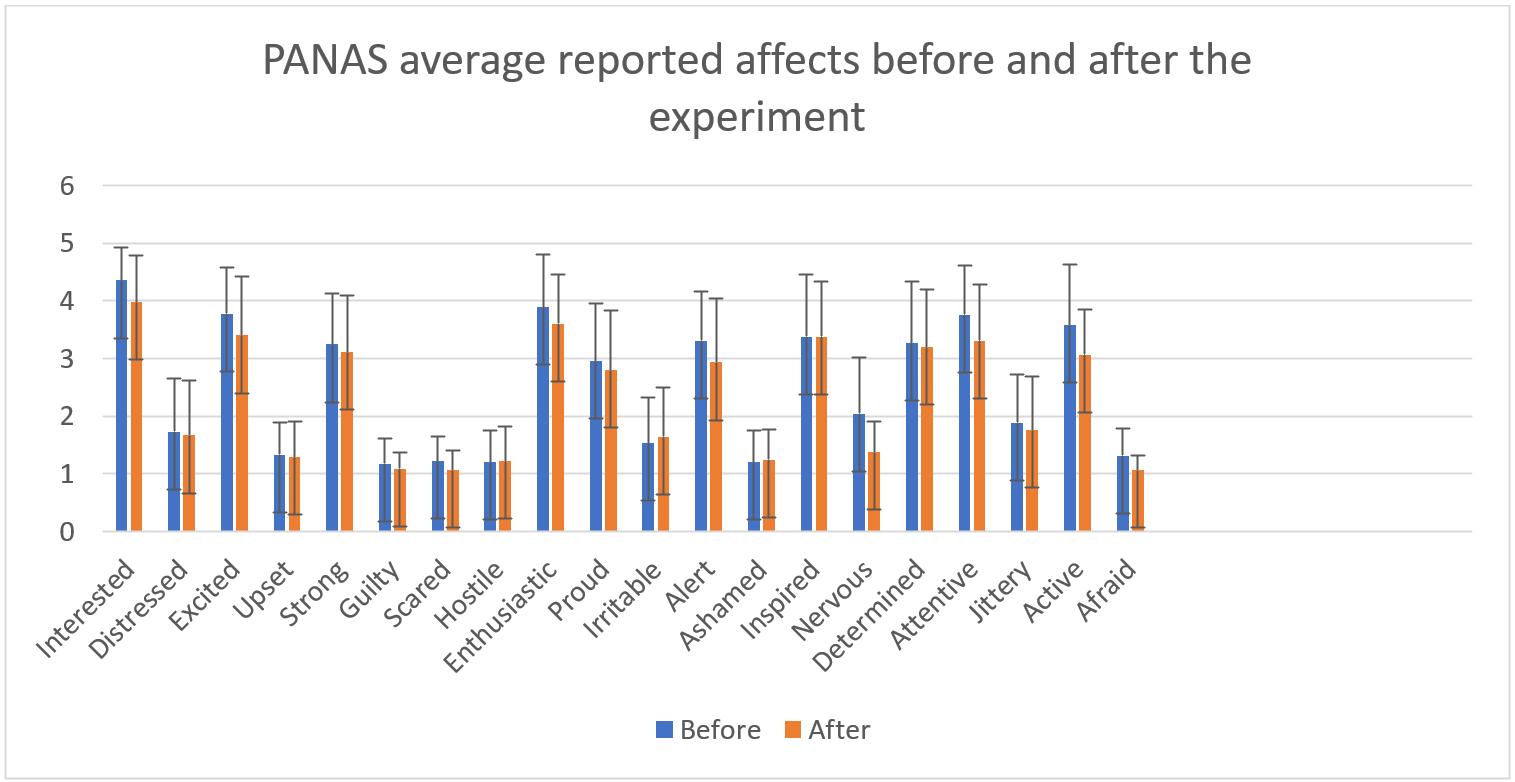
\includegraphics[width=12cm]{img/discussion/panas.png}
\centering
\caption{Average reported affects before and after the experimental session.} \label{fig:panas}
\end{figure}
Comparing the assessed affects before and after the experiment (Fig. \ref{fig:panas}), it is possible to observe that general interest, enthusiasm, and excitement of the participants decreased, which was expected considering that for the majority of the participants it was the first time participating in an EEG experiment. Attentiveness and activeness also significantly decreased, suggesting that the task proposed, and the length of the session were to some degree causing fatigue. Follow-up experiments can account for these effects by shortening the length of musical excerpts, reducing the number of conditions, or distributing the data collection from each participant over multiple sessions.

\section{Features selection and performances evaluation}
\label{sec:features_performances}
The proposed principal features based on previous findings on differential and rational asymmetries were the neuromarkers: \ac{AWI}, \ac{FMTI} and \ac{SASI}. The frequency-band specific features of the \ac{EEG} signal were extracted using the \ac{SPT} proprietary library from myBrainTechnologies. Intermediary experiments using forward \ac{SFS} revealed a general trend in selecting the neuromarkers as most significant features, with some exceptions. \ac{PCA} was then used instead of \ac{SFS} as better performing subject-dependent features selection method to reduce the dimensionality of the features vector in lower computational time. It was not possible to directly compare the impact of using neuromarkers instead of frequency-band specific features, but the results were very promising for a subset of participants. The evaluation of model performances using \ac{MCC} score led to better understanding and correcting models who were over-fitting toward the majority classes because of uneven distributions of labels. It made possible to easily identify under-fitting models too, however no solution was found to prevent it. Overall, \ac{MCC} score seems to be a more reliable score to describe the learning capabilities of the models, and it is better for comparison with the most recent related studies that make use of it, instead of classification accuracy only.

\section{From subject-dependent to subject-independent classification}
\label{sec:sd_to_si}
Clearly, subject-dependent classifiers are not an optimal solution for a real-time system and pose a threat to the usability by requiring full training sessions for new users. Besides, training a separated model for each user is not a long-term scalable solution. However, due to the subjective differences, subject-dependent remains the current preferred choice for Emotion-Recognition. Subject-independent strategy is only applicable to set of features that can represent the same emotional patterns for everyone, for example differential asymmetry was reported to be very promising \cite{lin_toward_2015}, but also assumes that all the datasets used for training are as clean as possible to prevent the contamination of artefacts. In the current study it was not possible to obtain better than default-guessing during intermediate experiments on subject-independent classification. Some conditions are likely to hinder classification:

\begin{itemize}
\item 	Artifacts: Data might be too affected by artifacts, hindering any classification.
\item 	Features: Selected features might not be suitable for all subjects, or they might be suitable only for groups of subjects with similar “brain signature”.
\item 	Labels: Distribution of the classes can be highly uneven, and self-reported labels can be unreliable.
\item 	Electrodes: Two electrodes might not contain sufficient significant data; they can be misplaced or bad conducting.
\end{itemize}
The enormous performance difference among subjects in subject-dependent classifications suggests that improvements in the first three conditions are not only possible, but also necessary towards the creation of wearable affective \ac{BCI}s. If the low number of electrodes were the main impediment to classification, it would not have been possible for some participants to score more than 80\% classification accuracy. After reducing the variability created by these conditions and once subject-dependent classification will yield consistent performances among subjects, it will be possible to further develop a hybrid paradigm where a subject-independent classifier serves as sub-optimal basis for fast calibration of subject-dependent classifiers. Finally, if these goals are met, full subject-independent classification will be the next step towards affective \ac{BCI}s.

\section{Reflections on future research}
\label{sec:future_research}
The analytical study of emotions is heavily impacted by subjective differences, and the current state of art technology and signal processing techniques still struggle to provide the desired performances to build seamless affective \ac{BCI} systems. Many critical factors starting from the data collection phase to the classification task can hinder the expected outcome. Considering the interest in a follow-up study, the factors that mainly affected the current study are addressed in the paragraphs below. 
\\
\\
\emph{Selection of the stimuli.} The selection of the stimuli is critical for the success for affective experiments, as there is nothing worse than selecting ineffective stimuli. Music is usually a favorable stimulus, since only a few subjects do not react at all to it. Even so, subjective preferences can highly impact the perception of the same song in a population of participants. This study conveniently “recycled” a selection of songs previously used in other experiments and proposed the same playlist to all participants for the sake of inter-subject comparison. This choice led the participants to a constrained experience, that for some resulted in listening to music genres they usually would not listen to. In addition, the annotation experience suffered of great variability, leading some subjects to never report some one or more valence-arousal classes. There are alternative solutions for the stimuli selection, as some related studies experimented \cite{thammasan_continuous_2016}. For example, the researcher can ask the subjects to pick music from a selection that covers the emotional spectrum during a pre-listening phase. A better compromise could be a hybrid selection: part of the stimuli selected by the researchers and the other part selected by the participants. Adapting the selection to account for the subjective preferences is very time consuming in the design of an experiment, but it is also what real users of an affective recommending system would expect.
\\
\\
\emph{Self-assessment of emotions.} As several participants reported, it was not always simple to assess in real-time perceived emotions, with the consequence of unreliable annotations. On one hand, knowing exactly what feelings are being experienced requires considerable self-perception. On the other hand, models for assessing emotions have limitations. As mentioned earlier (see Chapter \ref{sec:self_reported_labels} ), the \ac{VA} space used in the experiment was simplified to make it more understandable, sacrificing the representation of some emotional states. Using a more complete representation does not automatically improve the participants ability to report emotions, on the contrary it is likely to introduce more confusion. Other studies \cite{lin_eeg-based_2010} adopted an even more simplified version that only associates one emotion to each quadrant of the \ac{VA} space, that maybe partially explains the significantly better performances in classification. Continuous emotion annotations require more effort but are very valuable to capture emotion oscillations and provide classifiers with more realistic emotional distribution. Once the models for the classification of emotion will have reached maturity, continuous annotations will be discarded in favor of discrete reports, that better suit a real product. The solutions for Emotion-Recognition cannot possibly start from a complex representation of emotional states, thus building up from more simplified models might be a better strategy now to support the ongoing development of the field and then later scale up the complexity with more sophisticated tools.
\\
\\
\emph{Experimental sessions.} Two main observations were made based on the feedback received and the analysis of data. First one, a single session of 75-90 minutes (30-35 of \ac{EEG} recording) can be fatiguing for most people. Decreased attention and discomfort are not favorable conditions for recording brain activity and are likely to be reflected also on the emotional assessment. Second one, a single session does not ensure that classification performances are consistent for the same subject over time. External factors experienced prior to the session might bias the emotional perception of a subject, for example if there as a breakup with a loved one or if very good news brightened the day. In addition, the oscillatory nature of brain waves is known to generate differences in the \ac{EEG} signature of the same person over time. Multiple shorter session can prevent fatigue by reducing the overall mental load, and at the same time mitigate the effect of variations over time in the emotional assessment and in the \ac{EEG}.  
\\
\\
\emph{Automated lightweight preprocessing.} The requirements for a preprocessing pipeline in an online system are not easy to meet. Computational time needs to be in the order of seconds or even better milliseconds; at the same time the quality of data must be ensured to prevent poor classification performances. Ocular artifacts are the greatest threat in the analysis of emotions because of the topological position near the frontal lobe, where emotions are processed. Using \ac{EOG} to subtract eye movements from the EEG signal is effective for offline studies but is clearly not suitable for a product. Methods like \ac{ICA} and \ac{PCA} are very effective for \ac{EEG} recordings using standard equipment with many electrodes, but nevertheless computationally expensive. For a final product using wearable devices with limited capabilities, inferring the presence of artifacts by classifying \ac{EEG} based on the signal qualities \cite{grosselin_quality_2019} can be achieved with low computational effort and enable surgical precision in the cleaning process. \ac{ASR} has been proven effective in artifact removal for both offline data analysis and online applications \cite{chang_evaluation_2018}, but for optimal outcome, i.e. removing artifacts and retaining the significance of the signal, it requires to be tuned using good quality \ac{EEG} samples. Investigating the best combination of approaches for lightweight processing can be a suitable research question also outside the specific scope of affective \ac{BCI}.
\\
\\
\emph{Features extraction and selection.} Selecting the right features has proved to be non-trivial and affected by subject-dependent differences. The extraction process also carries a computation cost, thus just extracting any possible feature and then apply subjective selection criteria is not feasible. The current study used \ac{PCA} to collapse the features in the minimum number of components that could account for subjective differences and retain at least 95\% of the variability of the data. The neuromarkers are a step towards the delineation of an optimal subset of features for emotional assessment but require more investigation both from neuroscience and data science perspectives to determine which combination of differential/rational measurements and EEG frequency bands are more relevant for the study of emotions. The identification of more subject-independent features, like the asymmetry indexes \cite{lin_toward_2015}, is also essential towards the development of affective \ac{BCI} systems and can be the main topic of a dedicated research. The possibility to use other physiological signals to build a multi-modal classification system has also been explored, and physiological signals were collected during this research for eventual follow up studies. A related study already assessed the increased performances that can be obtained by decision-level multi-modal fusion \cite{thammasan_multimodal_2017}, an adaptive approach to select by majority voting the optimal uni-modal sources among several physiological measurements (\ac{EEG}, \ac{ECG}, \ac{GSR}) for classification. Any system designed on other physiological data than \ac{EEG} is, however, outside the strict scope of affective \ac{BCI}.
\\
\\
\emph{Unbalanced datasets.} One of the main obstacles in training and evaluating classification models was the uneven distribution of labels. Multiple experimental sessions and subjective stimuli selection can minimize the possibility of having very unbalanced datasets, as explained in the previous paragraph. However, it would still be possible to hit the same obstacle, regardless the minimization. In the field of machine learning there are standard methods to deal with unbalanced methods. Assigning weights to the classes to penalize the prediction of the majority class is one of such methods, used in the current to improve the discriminative power of \ac{SVM} classifiers. Up-sampling of the minority class is another method that creates copies of labels and data in the training dataset to reduce the bias of the classifier. However, copying affective data does not seem optimal as it would simply repeat the same emotional pattern and will not likely cover the entire emotional spectrum of the minority class. Some studies investigated the possibility of simulating realistic \ac{EEG} data \cite{barzegaran_eegsourcesim_2019} from biologically plausible signals. Good affective \ac{EEG} data from multiple subjects could be collected for the realization of a plausible \ac{EEG}  simulator that can account for individual variability. The data generator could then be calibrated over a small sample of real \ac{EEG}  data from a real subject and be used to counterbalance the distribution of emotional classes, thus improving the classification performances.
